

\tikzset{every picture/.style={line width=0.75pt}} %set default line width to 0.75pt        

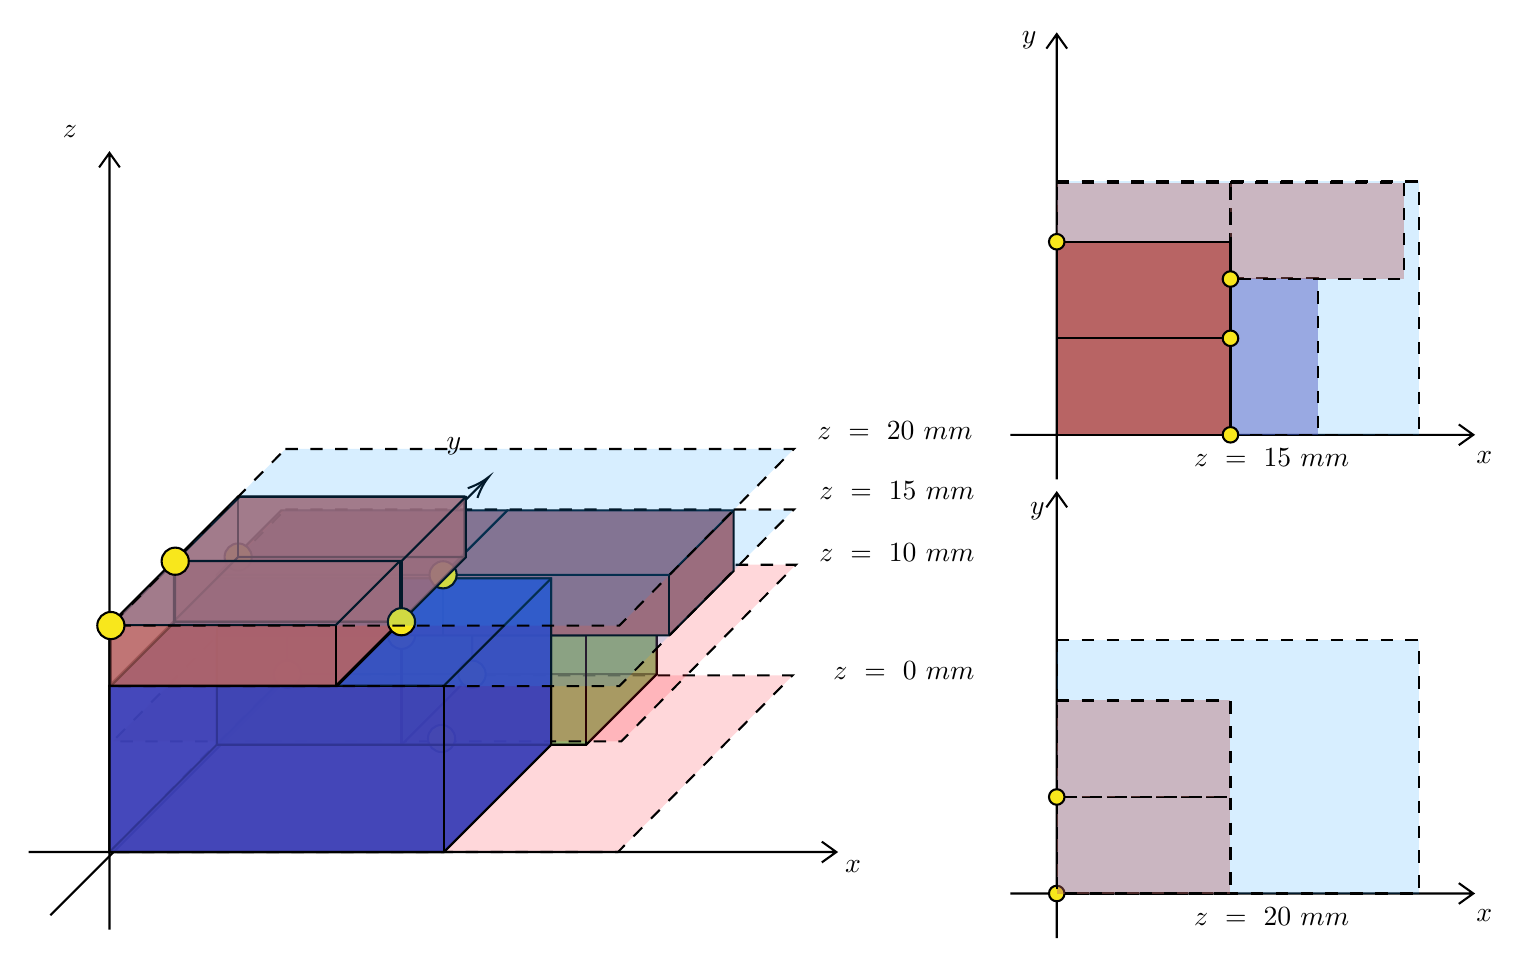
\begin{tikzpicture}[x=0.75pt,y=0.75pt,yscale=-1,xscale=1]
%uncomment if require: \path (0,517); %set diagram left start at 0, and has height of 517

%Shape: Cube [id:dp11750686891379902] 
\draw  [fill={rgb, 255:red, 130; green, 184; blue, 100 }  ,fill opacity=0.63 ] (420.59,331.37) -- (386.58,365.38) -- (297.6,365.38) -- (297.6,312.66) -- (331.6,278.65) -- (420.59,278.65) -- cycle ; \draw   (297.6,365.38) -- (331.6,331.37) -- (420.59,331.37) ; \draw   (331.6,331.37) -- (331.6,278.65) ;
%Shape: Parallelogram [id:dp761777526623073] 
\draw  [fill={rgb, 255:red, 255; green, 17; blue, 34 }  ,fill opacity=0.17 ][dash pattern={on 4.5pt off 4.5pt}] (241,332) -- (486,332) -- (401.91,417.07) -- (156.91,417.07) -- cycle ;
%Shape: Cube [id:dp9555955121552152] 
\draw  [fill={rgb, 255:red, 130; green, 184; blue, 100 }  ,fill opacity=0.63 ] (297.6,312.66) -- (331.6,278.65) -- (420.59,278.65) -- (420.59,331.37) -- (386.58,365.38) -- (297.6,365.38) -- cycle ; \draw   (420.59,278.65) -- (386.58,312.66) -- (297.6,312.66) ; \draw   (386.58,312.66) -- (386.58,365.38) ;
%Shape: Parallelogram [id:dp12159792926522017] 
\draw  [fill={rgb, 255:red, 255; green, 17; blue, 34 }  ,fill opacity=0.17 ][dash pattern={on 4.5pt off 4.5pt}] (242.62,278.65) -- (487.62,278.65) -- (403.53,363.73) -- (158.53,363.73) -- cycle ;
%Shape: Axis 2D [id:dp7547094969171453] 
\draw  (118,417.07) -- (507.11,417.07)(156.91,80.22) -- (156.91,454.5) (500.11,412.07) -- (507.11,417.07) -- (500.11,422.07) (151.91,87.22) -- (156.91,80.22) -- (161.91,87.22)  ;
%Straight Lines [id:da24486641728962577] 
\draw    (128.47,447.52) -- (338.19,237.8) ;
\draw [shift={(339.6,236.39)}, rotate = 135] [color={rgb, 255:red, 0; green, 0; blue, 0 }  ][line width=0.75]    (10.93,-3.29) .. controls (6.95,-1.4) and (3.31,-0.3) .. (0,0) .. controls (3.31,0.3) and (6.95,1.4) .. (10.93,3.29)   ;
%Shape: Cube [id:dp23740733074506637] 
\draw  [fill={rgb, 255:red, 130; green, 184; blue, 100 }  ,fill opacity=0.63 ] (331.6,331.37) -- (297.6,365.38) -- (208.61,365.38) -- (208.61,312.66) -- (242.62,278.65) -- (331.6,278.65) -- cycle ; \draw   (208.61,365.38) -- (242.62,331.37) -- (331.6,331.37) ; \draw   (242.62,331.37) -- (242.62,278.65) ;
%Shape: Cube [id:dp3377626309437859] 
\draw  [fill={rgb, 255:red, 130; green, 184; blue, 100 }  ,fill opacity=0.63 ] (208.61,312.66) -- (242.62,278.65) -- (331.6,278.65) -- (331.6,331.37) -- (297.6,365.38) -- (208.61,365.38) -- cycle ; \draw   (331.6,278.65) -- (297.6,312.66) -- (208.61,312.66) ; \draw   (297.6,312.66) -- (297.6,365.38) ;
%Shape: Ellipse [id:dp12890825920267357] 
\draw  [fill={rgb, 255:red, 248; green, 231; blue, 28 }  ,fill opacity=1 ] (236.07,331.37) .. controls (236.07,327.75) and (239,324.82) .. (242.62,324.82) .. controls (246.23,324.82) and (249.16,327.75) .. (249.16,331.37) .. controls (249.16,334.98) and (246.23,337.91) .. (242.62,337.91) .. controls (239,337.91) and (236.07,334.98) .. (236.07,331.37) -- cycle ;
%Shape: Axis 2D [id:dp22371680020517593] 
\draw  (591,216.05) -- (814,216.05)(613.3,23) -- (613.3,237.5) (807,211.05) -- (814,216.05) -- (807,221.05) (608.3,30) -- (613.3,23) -- (618.3,30)  ;
%Shape: Rectangle [id:dp19927589587496886] 
\draw  [fill={rgb, 255:red, 17; green, 154; blue, 255 }  ,fill opacity=0.17 ][dash pattern={on 4.5pt off 4.5pt}] (613.3,94) -- (788,94) -- (788,216.05) -- (613.3,216.05) -- cycle ;
%Shape: Rectangle [id:dp49701772163413693] 
\draw  [fill={rgb, 255:red, 61; green, 65; blue, 184 }  ,fill opacity=0.4 ][dash pattern={on 4.5pt off 4.5pt}] (613.3,140.5) -- (739,140.5) -- (739,216.05) -- (613.3,216.05) -- cycle ;
%Shape: Ellipse [id:dp9255158437533428] 
\draw  [fill={rgb, 255:red, 248; green, 231; blue, 28 }  ,fill opacity=1 ] (325.06,331.37) .. controls (325.06,327.75) and (327.99,324.82) .. (331.6,324.82) .. controls (335.22,324.82) and (338.15,327.75) .. (338.15,331.37) .. controls (338.15,334.98) and (335.22,337.91) .. (331.6,337.91) .. controls (327.99,337.91) and (325.06,334.98) .. (325.06,331.37) -- cycle ;
%Shape: Ellipse [id:dp7703154945024709] 
\draw  [fill={rgb, 255:red, 248; green, 231; blue, 28 }  ,fill opacity=1 ] (291.05,312.66) .. controls (291.05,309.05) and (293.98,306.12) .. (297.6,306.12) .. controls (301.21,306.12) and (304.14,309.05) .. (304.14,312.66) .. controls (304.14,316.28) and (301.21,319.21) .. (297.6,319.21) .. controls (293.98,319.21) and (291.05,316.28) .. (291.05,312.66) -- cycle ;
%Shape: Ellipse [id:dp2590138006968361] 
\draw  [fill={rgb, 255:red, 248; green, 231; blue, 28 }  ,fill opacity=1 ] (310.37,362.37) .. controls (310.37,358.76) and (313.3,355.83) .. (316.91,355.83) .. controls (320.52,355.83) and (323.45,358.76) .. (323.45,362.37) .. controls (323.45,365.98) and (320.52,368.91) .. (316.91,368.91) .. controls (313.3,368.91) and (310.37,365.98) .. (310.37,362.37) -- cycle ;
%Shape: Cube [id:dp2760918772938089] 
\draw  [fill={rgb, 255:red, 184; green, 100; blue, 100 }  ,fill opacity=1 ] (208.61,283.5) -- (239.61,252.5) -- (348.63,252.5) -- (348.63,281.66) -- (317.63,312.66) -- (208.61,312.66) -- cycle ; \draw   (348.63,252.5) -- (317.63,283.5) -- (208.61,283.5) ; \draw   (317.63,283.5) -- (317.63,312.66) ;
%Shape: Cube [id:dp25888946519283873] 
\draw  [fill={rgb, 255:red, 184; green, 100; blue, 100 }  ,fill opacity=1 ] (317.63,283.5) -- (348.63,252.5) -- (457.65,252.5) -- (457.65,281.66) -- (426.65,312.66) -- (317.63,312.66) -- cycle ; \draw   (457.65,252.5) -- (426.65,283.5) -- (317.63,283.5) ; \draw   (426.65,283.5) -- (426.65,312.66) ;
%Shape: Cube [id:dp5116746047827113] 
\draw  [fill={rgb, 255:red, 61; green, 65; blue, 184 }  ,fill opacity=0.8 ] (369.7,365.38) -- (318,417.07) -- (156.91,417.07) -- (156.91,336.94) -- (208.61,285.25) -- (369.7,285.25) -- cycle ; \draw   (156.91,417.07) -- (208.61,365.38) -- (369.7,365.38) ; \draw   (208.61,365.38) -- (208.61,285.25) ;
%Shape: Cube [id:dp9793419692541124] 
\draw  [fill={rgb, 255:red, 61; green, 65; blue, 184 }  ,fill opacity=0.8 ] (156.91,336.94) -- (208.61,285.25) -- (369.7,285.25) -- (369.7,365.38) -- (318,417.07) -- (156.91,417.07) -- cycle ; \draw   (369.7,285.25) -- (318,336.94) -- (156.91,336.94) ; \draw   (318,336.94) -- (318,417.07) ;
%Shape: Parallelogram [id:dp012772412734990968] 
\draw  [fill={rgb, 255:red, 17; green, 154; blue, 255 }  ,fill opacity=0.17 ][dash pattern={on 4.5pt off 4.5pt}] (241.66,252.05) -- (486.66,252.05) -- (402.57,337.12) -- (157.57,337.12) -- cycle ;
%Shape: Rectangle [id:dp19856633465195028] 
\draw  [fill={rgb, 255:red, 184; green, 100; blue, 100 }  ,fill opacity=0.4 ][dash pattern={on 4.5pt off 4.5pt}] (613.3,94.5) -- (697,94.5) -- (697,141) -- (613.3,141) -- cycle ;
%Shape: Rectangle [id:dp9568505376978227] 
\draw  [fill={rgb, 255:red, 184; green, 100; blue, 100 }  ,fill opacity=0.4 ][dash pattern={on 4.5pt off 4.5pt}] (697,94.5) -- (780.7,94.5) -- (780.7,141) -- (697,141) -- cycle ;
%Shape: Axis 2D [id:dp905993353659617] 
\draw  (591,437.05) -- (814,437.05)(613.3,244) -- (613.3,458.5) (807,432.05) -- (814,437.05) -- (807,442.05) (608.3,251) -- (613.3,244) -- (618.3,251)  ;
%Shape: Rectangle [id:dp7116456668997998] 
\draw  [fill={rgb, 255:red, 17; green, 154; blue, 255 }  ,fill opacity=0.17 ][dash pattern={on 4.5pt off 4.5pt}] (613.3,315) -- (788,315) -- (788,437.05) -- (613.3,437.05) -- cycle ;
%Shape: Circle [id:dp6552301353176846] 
\draw  [fill={rgb, 255:red, 248; green, 231; blue, 28 }  ,fill opacity=1 ] (609.55,437.05) .. controls (609.55,434.98) and (611.23,433.3) .. (613.3,433.3) .. controls (615.37,433.3) and (617.05,434.98) .. (617.05,437.05) .. controls (617.05,439.12) and (615.37,440.8) .. (613.3,440.8) .. controls (611.23,440.8) and (609.55,439.12) .. (609.55,437.05) -- cycle ;
%Shape: Rectangle [id:dp45682836776869995] 
\draw  [fill={rgb, 255:red, 184; green, 100; blue, 100 }  ,fill opacity=0.4 ][dash pattern={on 4.5pt off 4.5pt}] (613.3,390.55) -- (697,390.55) -- (697,437.05) -- (613.3,437.05) -- cycle ;
%Shape: Rectangle [id:dp057027447735892856] 
\draw  [fill={rgb, 255:red, 184; green, 100; blue, 100 }  ,fill opacity=1 ] (613.3,169.55) -- (697,169.55) -- (697,216.05) -- (613.3,216.05) -- cycle ;
%Shape: Circle [id:dp893710699889989] 
\draw  [fill={rgb, 255:red, 248; green, 231; blue, 28 }  ,fill opacity=1 ] (693.25,216.05) .. controls (693.25,213.98) and (694.93,212.3) .. (697,212.3) .. controls (699.07,212.3) and (700.75,213.98) .. (700.75,216.05) .. controls (700.75,218.12) and (699.07,219.8) .. (697,219.8) .. controls (694.93,219.8) and (693.25,218.12) .. (693.25,216.05) -- cycle ;
%Shape: Ellipse [id:dp6797422863626328] 
\draw  [fill={rgb, 255:red, 248; green, 231; blue, 28 }  ,fill opacity=1 ] (212.37,274.94) .. controls (212.37,271.33) and (215.3,268.4) .. (218.91,268.4) .. controls (222.52,268.4) and (225.45,271.33) .. (225.45,274.94) .. controls (225.45,278.56) and (222.52,281.49) .. (218.91,281.49) .. controls (215.3,281.49) and (212.37,278.56) .. (212.37,274.94) -- cycle ;
%Shape: Ellipse [id:dp1667953327037479] 
\draw  [fill={rgb, 255:red, 248; green, 231; blue, 28 }  ,fill opacity=1 ] (311.09,283.5) .. controls (311.09,279.89) and (314.02,276.96) .. (317.63,276.96) .. controls (321.24,276.96) and (324.17,279.89) .. (324.17,283.5) .. controls (324.17,287.11) and (321.24,290.04) .. (317.63,290.04) .. controls (314.02,290.04) and (311.09,287.11) .. (311.09,283.5) -- cycle ;
%Shape: Cube [id:dp8379525701182935] 
\draw  [fill={rgb, 255:red, 184; green, 100; blue, 100 }  ,fill opacity=0.67 ] (297.6,306.12) -- (266.6,337.12) -- (157.57,337.12) -- (157.57,307.96) -- (188.57,276.96) -- (297.6,276.96) -- cycle ; \draw   (157.57,337.12) -- (188.57,306.12) -- (297.6,306.12) ; \draw   (188.57,306.12) -- (188.57,276.96) ;
%Shape: Cube [id:dp526221096875487] 
\draw  [fill={rgb, 255:red, 184; green, 100; blue, 100 }  ,fill opacity=0.67 ] (327.93,274.94) -- (296.93,305.94) -- (187.91,305.94) -- (187.91,276.78) -- (218.91,245.78) -- (327.93,245.78) -- cycle ; \draw   (187.91,305.94) -- (218.91,274.94) -- (327.93,274.94) ; \draw   (218.91,274.94) -- (218.91,245.78) ;
%Shape: Cube [id:dp19903463769753094] 
\draw  [fill={rgb, 255:red, 184; green, 100; blue, 100 }  ,fill opacity=0.67 ] (188.57,276.96) -- (219.57,245.96) -- (328.6,245.96) -- (328.6,275.12) -- (297.6,306.12) -- (188.57,306.12) -- cycle ; \draw   (328.6,245.96) -- (297.6,276.96) -- (188.57,276.96) ; \draw   (297.6,276.96) -- (297.6,306.12) ;
%Shape: Cube [id:dp8602856031053141] 
\draw  [fill={rgb, 255:red, 184; green, 100; blue, 100 }  ,fill opacity=0.67 ] (156.91,307.78) -- (187.91,276.78) -- (296.93,276.78) -- (296.93,305.94) -- (265.93,336.94) -- (156.91,336.94) -- cycle ; \draw   (296.93,276.78) -- (265.93,307.78) -- (156.91,307.78) ; \draw   (265.93,307.78) -- (265.93,336.94) ;
%Shape: Ellipse [id:dp4815406681346305] 
\draw  [fill={rgb, 255:red, 248; green, 231; blue, 28 }  ,fill opacity=1 ] (291.05,306.12) .. controls (291.05,302.51) and (293.98,299.58) .. (297.6,299.58) .. controls (301.21,299.58) and (304.14,302.51) .. (304.14,306.12) .. controls (304.14,309.73) and (301.21,312.66) .. (297.6,312.66) .. controls (293.98,312.66) and (291.05,309.73) .. (291.05,306.12) -- cycle ;
%Shape: Parallelogram [id:dp8761855833958668] 
\draw  [fill={rgb, 255:red, 17; green, 154; blue, 255 }  ,fill opacity=0.17 ][dash pattern={on 4.5pt off 4.5pt}] (241.66,222.88) -- (486.66,222.88) -- (402.57,307.96) -- (157.57,307.96) -- cycle ;
%Shape: Ellipse [id:dp18311715249003535] 
\draw  [fill={rgb, 255:red, 248; green, 231; blue, 28 }  ,fill opacity=1 ] (151.03,307.96) .. controls (151.03,304.34) and (153.96,301.41) .. (157.57,301.41) .. controls (161.19,301.41) and (164.12,304.34) .. (164.12,307.96) .. controls (164.12,311.57) and (161.19,314.5) .. (157.57,314.5) .. controls (153.96,314.5) and (151.03,311.57) .. (151.03,307.96) -- cycle ;
%Shape: Ellipse [id:dp8613169128999868] 
\draw  [fill={rgb, 255:red, 248; green, 231; blue, 28 }  ,fill opacity=1 ] (182.03,276.96) .. controls (182.03,273.34) and (184.96,270.41) .. (188.57,270.41) .. controls (192.19,270.41) and (195.12,273.34) .. (195.12,276.96) .. controls (195.12,280.57) and (192.19,283.5) .. (188.57,283.5) .. controls (184.96,283.5) and (182.03,280.57) .. (182.03,276.96) -- cycle ;
%Shape: Rectangle [id:dp49121416555728614] 
\draw  [fill={rgb, 255:red, 184; green, 100; blue, 100 }  ,fill opacity=0.4 ][dash pattern={on 4.5pt off 4.5pt}] (613.3,344.05) -- (697,344.05) -- (697,390.55) -- (613.3,390.55) -- cycle ;
%Shape: Circle [id:dp8077543912869247] 
\draw  [fill={rgb, 255:red, 248; green, 231; blue, 28 }  ,fill opacity=1 ] (609.55,390.55) .. controls (609.55,388.48) and (611.23,386.8) .. (613.3,386.8) .. controls (615.37,386.8) and (617.05,388.48) .. (617.05,390.55) .. controls (617.05,392.62) and (615.37,394.3) .. (613.3,394.3) .. controls (611.23,394.3) and (609.55,392.62) .. (609.55,390.55) -- cycle ;
%Shape: Rectangle [id:dp4869036595737919] 
\draw  [fill={rgb, 255:red, 184; green, 100; blue, 100 }  ,fill opacity=1 ] (613.3,123.05) -- (697,123.05) -- (697,169.55) -- (613.3,169.55) -- cycle ;
%Shape: Circle [id:dp883887984988515] 
\draw  [fill={rgb, 255:red, 248; green, 231; blue, 28 }  ,fill opacity=1 ] (693.25,141) .. controls (693.25,138.93) and (694.93,137.25) .. (697,137.25) .. controls (699.07,137.25) and (700.75,138.93) .. (700.75,141) .. controls (700.75,143.07) and (699.07,144.75) .. (697,144.75) .. controls (694.93,144.75) and (693.25,143.07) .. (693.25,141) -- cycle ;
%Shape: Circle [id:dp6519707767315044] 
\draw  [fill={rgb, 255:red, 248; green, 231; blue, 28 }  ,fill opacity=1 ] (693.25,169.55) .. controls (693.25,167.48) and (694.93,165.8) .. (697,165.8) .. controls (699.07,165.8) and (700.75,167.48) .. (700.75,169.55) .. controls (700.75,171.62) and (699.07,173.3) .. (697,173.3) .. controls (694.93,173.3) and (693.25,171.62) .. (693.25,169.55) -- cycle ;
%Shape: Circle [id:dp6617436886058339] 
\draw  [fill={rgb, 255:red, 248; green, 231; blue, 28 }  ,fill opacity=1 ] (609.55,123.05) .. controls (609.55,120.98) and (611.23,119.3) .. (613.3,119.3) .. controls (615.37,119.3) and (617.05,120.98) .. (617.05,123.05) .. controls (617.05,125.12) and (615.37,126.8) .. (613.3,126.8) .. controls (611.23,126.8) and (609.55,125.12) .. (609.55,123.05) -- cycle ;

% Text Node
\draw (504.19,323.66) node [anchor=north west][inner sep=0.75pt]    {$z\ =\ 0\ mm$};
% Text Node
\draw (317.9,215.7) node [anchor=north west][inner sep=0.75pt]    {$y$};
% Text Node
\draw (509.84,419.85) node [anchor=north west][inner sep=0.75pt]    {$x$};
% Text Node
\draw (132.94,65.64) node [anchor=north west][inner sep=0.75pt]    {$z$};
% Text Node
\draw (497.48,237.2) node [anchor=north west][inner sep=0.75pt]    {$z\ =\ 15\ mm$};
% Text Node
\draw (814,222.4) node [anchor=north west][inner sep=0.75pt]    {$x$};
% Text Node
\draw (678,221.4) node [anchor=north west][inner sep=0.75pt]    {$z\ =\ 15\ mm$};
% Text Node
\draw (497.48,267.2) node [anchor=north west][inner sep=0.75pt]    {$z\ =\ 10\ mm$};
% Text Node
\draw (496.48,208.2) node [anchor=north west][inner sep=0.75pt]    {$z\ =\ 20\ mm$};
% Text Node
\draw (814,443.4) node [anchor=north west][inner sep=0.75pt]    {$x$};
% Text Node
\draw (678,442.4) node [anchor=north west][inner sep=0.75pt]    {$z\ =\ 20\ mm$};
% Text Node
\draw (595,20.4) node [anchor=north west][inner sep=0.75pt]    {$y$};
% Text Node
\draw (599,247.4) node [anchor=north west][inner sep=0.75pt]    {$y$};


\end{tikzpicture}
